\chapter{ANÁLISIS DE RESULTADOS}
Una vez que se establece el diseño a seguir en este TFM, se pasa a realizar el análisis de resultados.

Este análisis de resultados diferencia entre aquellos resultados obtenidos en el análisis exploratorio y los obtenidos en la aplicación de modelos predictivos.

\section{Análisis exploratorio de datos}

Antes de comenzar con el análisis, el lector puede observar en la tabla \ref{tab:TablaVariables} del Apéndice \ref{appendix:A} las variables utilizadas en esta investigación. En este mismo Anexo nos encontramos también los estadísticos, que se pueden observar en la figura \ref{fig:estadisticos}.

\begin{figure*}[htb]
	\centering
	\caption{Estadísticos de las variables. Elaboración propia}
	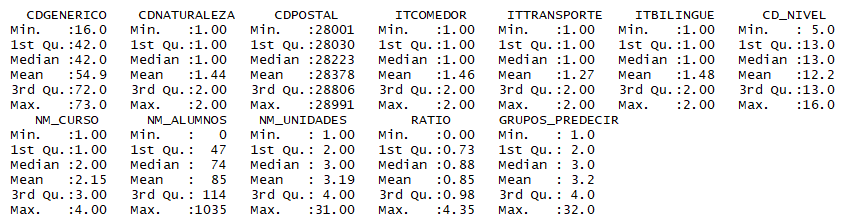
\includegraphics[width=1\textwidth]{recursos/ImagenesR/estadisticos}
	\label{fig:estadisticos}
\end{figure*}
\FloatBarrier

Una de los estadísticos más relevantes que se pueden apreciar en la figura \ref{fig:estadisticos} es la media de la variable ratio, que es de 0,88 y menor que 1. Esto implica que los centros de la Comunidad de Madrid no están sobrepoblados.

Una vez observados los estadísticos, los vamos a representar utilizando los diagramas de caja (box-plot). Con estos diagramas vamos a observar además los datos atípicos (outliers). Un resumen de todos los diagramas de cajas se puede observar en la figura \ref{fig:boxplotNorm}.

\begin{figure*}[htb]
	\centering
	\caption{Diagrama de cajas normalizado. Elaboración propia}
	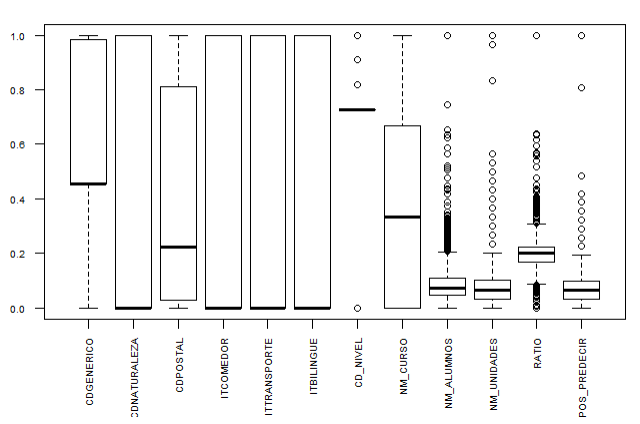
\includegraphics[width=0.8\textwidth]{recursos/ImagenesR/boxplotNorm}
	\label{fig:boxplotNorm}
\end{figure*}



Como se puede observar en la figura \ref{fig:boxplotNorm}, las variables de número de alumnos, número de unidades y ratio contienen datos anómalos. Por ejemplo, la variable número de alumnos (nm\_alumnos), como se puede apreciar en los estadísticos de la figura \ref{fig:estadisticos} tiene una media de 74 alumnos. No obstante, hay niveles educativos que tienen hasta casi 700 alumnos. Esto se debe a que los centros relativos a estos alumnos tienen la modalidad de distancia para esos niveles educativos, esto implica que pueden tener un gran número de unidades debido al gran número de alumnos que se matriculan para esta modalidad. Ocurre, por tanto, exactamente lo mismo con el número de grupos y la ratio. Estos datos anómalos no se van a eliminar puesto que tienen sentido en esta investigación.

Una vez estudiados los estadísticos y los datos anómalos, se realiza un estudio sobre la normalidad de los datos. En este aspecto es importante destacar que después de realizar el test de Mardia se observa que los datos utilizados rechazan la hipótesis de normalidad. Este rechazo implica una mayor cota de error a la hora de predecir los datos. Además, existen determinados modelos predictivos que no asumen que sus datos provengan de determinadas distribuciones. Véase el Anexo \ref{appendix:AB1}

Posteriormente se realiza un estudio sobre aquellas unidades que tuvieran la ratio superior a 1 (implica que hay una sobrepoblación en el aula). En la figura \ref{fig:histDat} se puede observar como la DAT-Centro (5) es la que mayor sobrepoblación tiene seguida de la DAT-Sur. Esta situación quizá sea por la falta de recursos o la sobrepoblación de la zona.

\begin{figure*}[htb]
	\centering
	\caption{Dirección de Área Territorial con aulas sobrepobladas. Elaboración propia}
	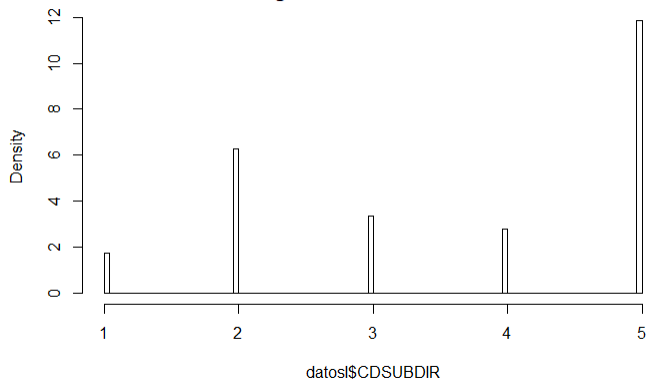
\includegraphics[width=0.6\textwidth]{recursos/ImagenesR/histDat}
	\label{fig:histDat}
\end{figure*}
\FloatBarrier

\begin{figure*}[htb]
	\centering
	\caption{Distribución de variables cuando existe sobrepoblación. Elaboración propia}
	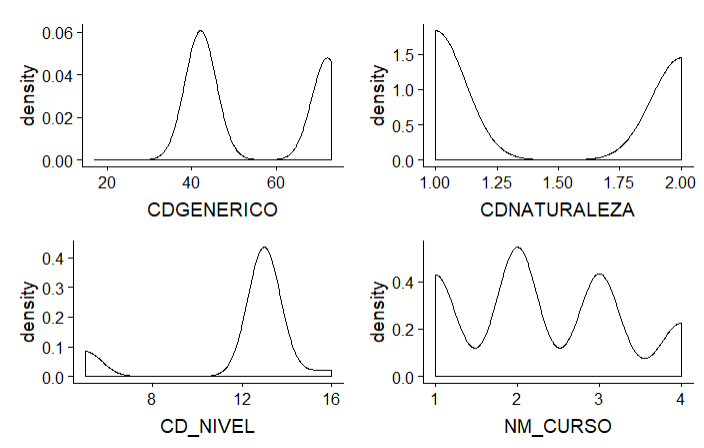
\includegraphics[width=0.8\textwidth]{recursos/ImagenesR/DistSobrepoblacion}
	\label{fig:DistSobrepoblacion}
\end{figure*}
\FloatBarrier

En la figura \ref{fig:DistSobrepoblacion} puede observarse que cuando existe sobrepoblación en el aula, suele ocurrir en centros públicos, mas que en centros privados. Además, suele darse en los niveles de la ESO. Para cada nivel, dentro de los cursos existentes, la sobrepoblación se da para el segundo curso. Por ej: 2º ESO, 2º Bachillerato, etc. Por tanto, la sobrepoblación suele darse en el segundo curso de la ESO. Esto puede deberse al numero de repetidores.

Uno de los aspectos más importantes en el análisis exploratorio de datos es la correlación existente entre las variables. En la figura \ref{fig:matrizcorrelaciones} se puede observar como existe una gran correlación entre las variables número de alumnos, número de grupos y grupos a predecir y otra gran correlación entre la variable comedor, el carácter genérico y la naturaleza del centro. 

Otras relaciones observadas es que, como cabe esperar, el numero de unidades tiene una gran relación con las unidades a predecir. Véase la figura \ref{fig:RelacionGruposYUnidades} del Anexo \ref{appendix:AB2}

En la figura \ref{fig:mayorescorrelaciones} se pueden observar las mayores correlaciones entre variables ordenadas de mayor a menor.

\begin{figure*}[htb]
	\centering
	\caption{Matriz de correlaciones. Elaboración propia}
	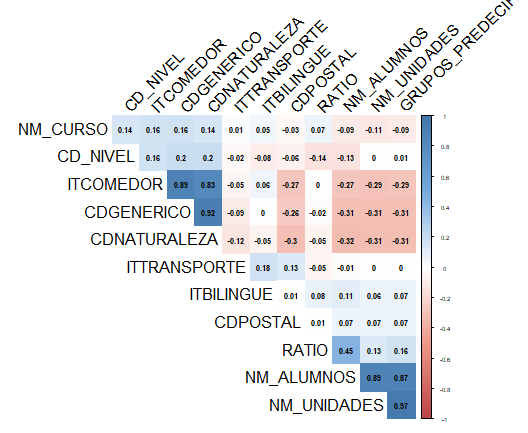
\includegraphics[width=0.8\textwidth]{recursos/ImagenesR/matrizcorrelacion}
	\label{fig:matrizcorrelaciones}
\end{figure*}

\begin{figure*}[htb]
	\centering
	\caption{Variables más correladas. Elaboración propia}
	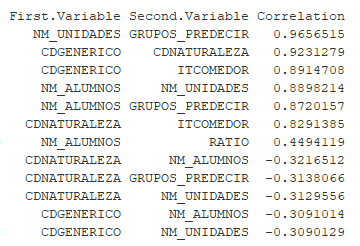
\includegraphics[width=0.6\textwidth]{recursos/ImagenesR/mayorescorrelaciones}
	\label{fig:mayorescorrelaciones}
\end{figure*}


\begin{figure*}[htb]
	\centering
	\caption{Mayor correlación con variable a predecir. Elaboración propia}
	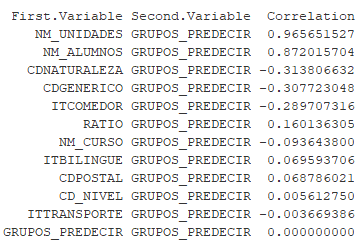
\includegraphics[width=0.6\textwidth]{recursos/ImagenesR/mayorcorrelacion}
	\label{fig:mayorcorrelacionpredecir}
\end{figure*}


En las figuras \ref{fig:matrizcorrelaciones}, \ref{fig:mayorescorrelaciones} y \ref{fig:mayorcorrelacionpredecir} se muestra prácticamente la misma información, la correlación entre variables. En la figura \ref{fig:mayorescorrelaciones} se muestran aquellos pares de variables que poseen la mayor correlación. Se puede apreciar en esta figura que la variable numero de unidades y grupos a predecir tienen una correlación casi perfecta, lo que implica que aportarían la misma información al conjunto de datos.

En la figura \ref{fig:mayorcorrelacionpredecir} se muestran aquellas variables que tienen mayor correlación con la variable a predecir. Podemos observar que las variables de numero de unidades y numero de alumnos tienen una enorme correlación con la variable a predecir. Esta relación es lógica, ya que, a mayor número de alumnos o grupos, la variable a predecir aumenta.  No sorprende puesto que son variables determinantes en la predicción. También se puede destacar que la naturaleza (pública o privada) de un centro está relacionada con el número de grupos a predecir. Al aumentar el valor de la naturaleza, disminuye el número de unidades. De esta premisa se puede deducir que los padres tienden a matricular a sus hijos en centros públicos, y, por lo tanto, el número de grupos tiende a aumentar. %El servicio de comedor también es un factor con relación con el número de grupos, lo que implica que los padres suelen matricular a los alumnos en centros que dispongan de este servicio.

También nos interesa saber las variables que están correlacionadas con la ratio, entre estas variables nos encontramos con una correlación positiva bastante fuerte el número de alumnos. Si el número de alumnos crece, la ratio va a crecer obligatoriamente (mientras no se creen nuevos centros). También se puede destacar el servicio de comedor, que tiene una correlación negativa, lo que implica que las aulas con sobrepoblación son aquellas cuyo centro no ofrece un servicio de comedor. Este resultado se debe a que los centros de secundaria que suelen tener servicio de comedor, suelen ser centros privados, y, por lo tanto, suelen tener las ratios por debajo de 1. Lo mismo ocurre con otras variables como la naturaleza o el código genérico. Véase la figura \ref{fig:variablesRatio}

\begin{figure*}[htb]
	\centering
	\caption{Mayores correlaciones con la Ratio. Elaboración propia}
	\includegraphics[width=0.8\textwidth]{recursos/ImagenesR/variablesRatio}
	\label{fig:variablesRatio}
\end{figure*}
\FloatBarrier


Una vez obtenidos los resultados del análisis exploratorio, se muestran los resultados obtenidos en el análisis predictivo.

\section{Análisis predictivo}
En primer lugar, debe tenerse en cuenta que todas las variables comentadas no tienen la misma trascendencia en el resultado. Para detectar esta relevancia de variables se utilizan técnicas que muestren dichas variables. Utilizando Random Forest, en la figura \ref{fig:VarImpRF} del Anexo \ref{appendix:AC1} podemos observar que las más importantes a la hora de mejorar la precisión en el modelo son: el número de unidades y alumnos.

En cambio, se ha utilizado el algoritmo de Regresión Paso a Paso y se ha obtenido que se utilizan como máximo 5 variables (naturaleza del centro, numero de curso, número de unidades, nivel de enseñanza y ratio). Utilizando estas variables es cuando el modelo obtiene la mayor precisión. Son, por tanto, variables importantes en este estudio. El resto de variables aportan en la predicción, pero muy poco, por consiguiente, consideramos que no son variables que tengan influencia en la sobrepoblación del aula. Véase el Anexo \ref{appendix:A.C.2} para más información.

%En primer lugar, se debe tener en cuenta las variables que se van a utilizar en los modelos, para ello, se va a utilizar Random Forest como algoritmo para obtener la importancia de las variables. En la figura \ref{fig:VarImpRF} podemos observar que las vas importantes a la hora de mejorar la precisión en el modelo son: número de unidades y alumnos.

%Se utiliza también otro algoritmo que es el conocido como Regresión Paso a Paso. Para este algoritmo se utilizan 3 estrategias en este TFM. En las estrategias descritas en el Apéndice \ref{appendix:A.C.2} resultando que dos de estas estrategias utilizan como máximo 5 variables (naturaleza del centro, numero de curso, número de unidades, nivel de enseñanza y ratio). Estas variables se tienen en cuenta para la realización y comparación de modelos. Utilizando estas variables es cuando el modelo obtiene la mayor precisión. Debe destacarse que la mayoría de estas variables son las que mayor correlación tienen con la variable a predecir.

%En esta investigación, además de realizar la comparación de los modelos, también se va a realizar una comparación teniendo en cuenta todas las variables y únicamente las 5 variables seleccionadas utilizando los algoritmos, ya comentados, de eliminación de variables.

%Los resultados obtenidos, que pueden observarse en la tabla \ref{tab:ComparacionModelos} en el Apéndice \ref{appendix:B} puede observarse como el algoritmo que mayor precisión ha obtenido ha sido el Árbol de decisión utilizando todas las variables. No obstante, este algoritmo requiere de un gran tiempo de entrenamiento, por lo que la regresión lineal puede ser una gran opción. Como puede observarse en el figura \ref{fig:ComparacionModelosII} del Apéndice \ref{appendix:B} existen varios modelos que obtienen precisiones similares (Redes neuronales, Árbol de Decisión y Regresión Linear) por tanto es conveniente tener en cuenta los tiempo de entrenamiento que se pueden ver en la figura \ref{fig:ComparacionModelosTiempo}.

%En una nueva investigación se debe tener en cuenta el tiempo de entrenamiento, sin embargo, como ya se ha realizado el entrenamiento, se va a obtener la predicción utilizando el algoritmo de Árbol de decisión (xgbTree). 

Una vez seleccionado el algoritmo a usar en la predicción (árbol de decisión), se puede observar una situación que realmente ocurre, y es que pocos centros son los que aumentan o disminuyen de unidades. Concretamente, de 4436 datos con los que se trabajan, únicamente 52 cambian. Algunos de estos grupos se observan en la figura \ref{fig:UnidadesDistintasPrediccion}.

\begin{figure*}[htb]
	\centering
	\caption{Aumento o disminución de grupos en la predicción. Elaboración propia}
	\label{fig:UnidadesDistintasPrediccion}
	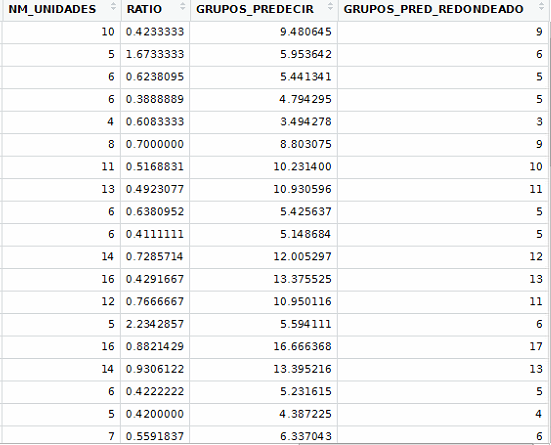
\includegraphics[width=0.6\textwidth]{recursos/ImagenesR/UnidadesDistintasPrediccion}
\end{figure*}
\FloatBarrier

De estos 52 grupos que cambian: 30 de ellos son grupos que van a disminuir su número y el restante 22, son grupos que van a aumentar su número. Esto podría deberse a una posible despoblación de la zona en la que se encuentran dichos centros.





